\section{The Player(s)}
\label{sec:players}

The Player Agents within are implemented as \emph{modular BDI shells}, acting as an interface wrapper around a \emph{Reasoner}, whose exact behavior must be implemented by the developer. This architecture cleanly decouples the network communication and state management from the actual decision-making logic.

As illustrated in Figure \ref{fig:agent_interface}, the agent shell exposes two primary interfaces to interact with the environment: a \emph{Decision Execution Interface} and a \emph{State Management Interface}.

\begin{figure}[htpb]
    \centering
    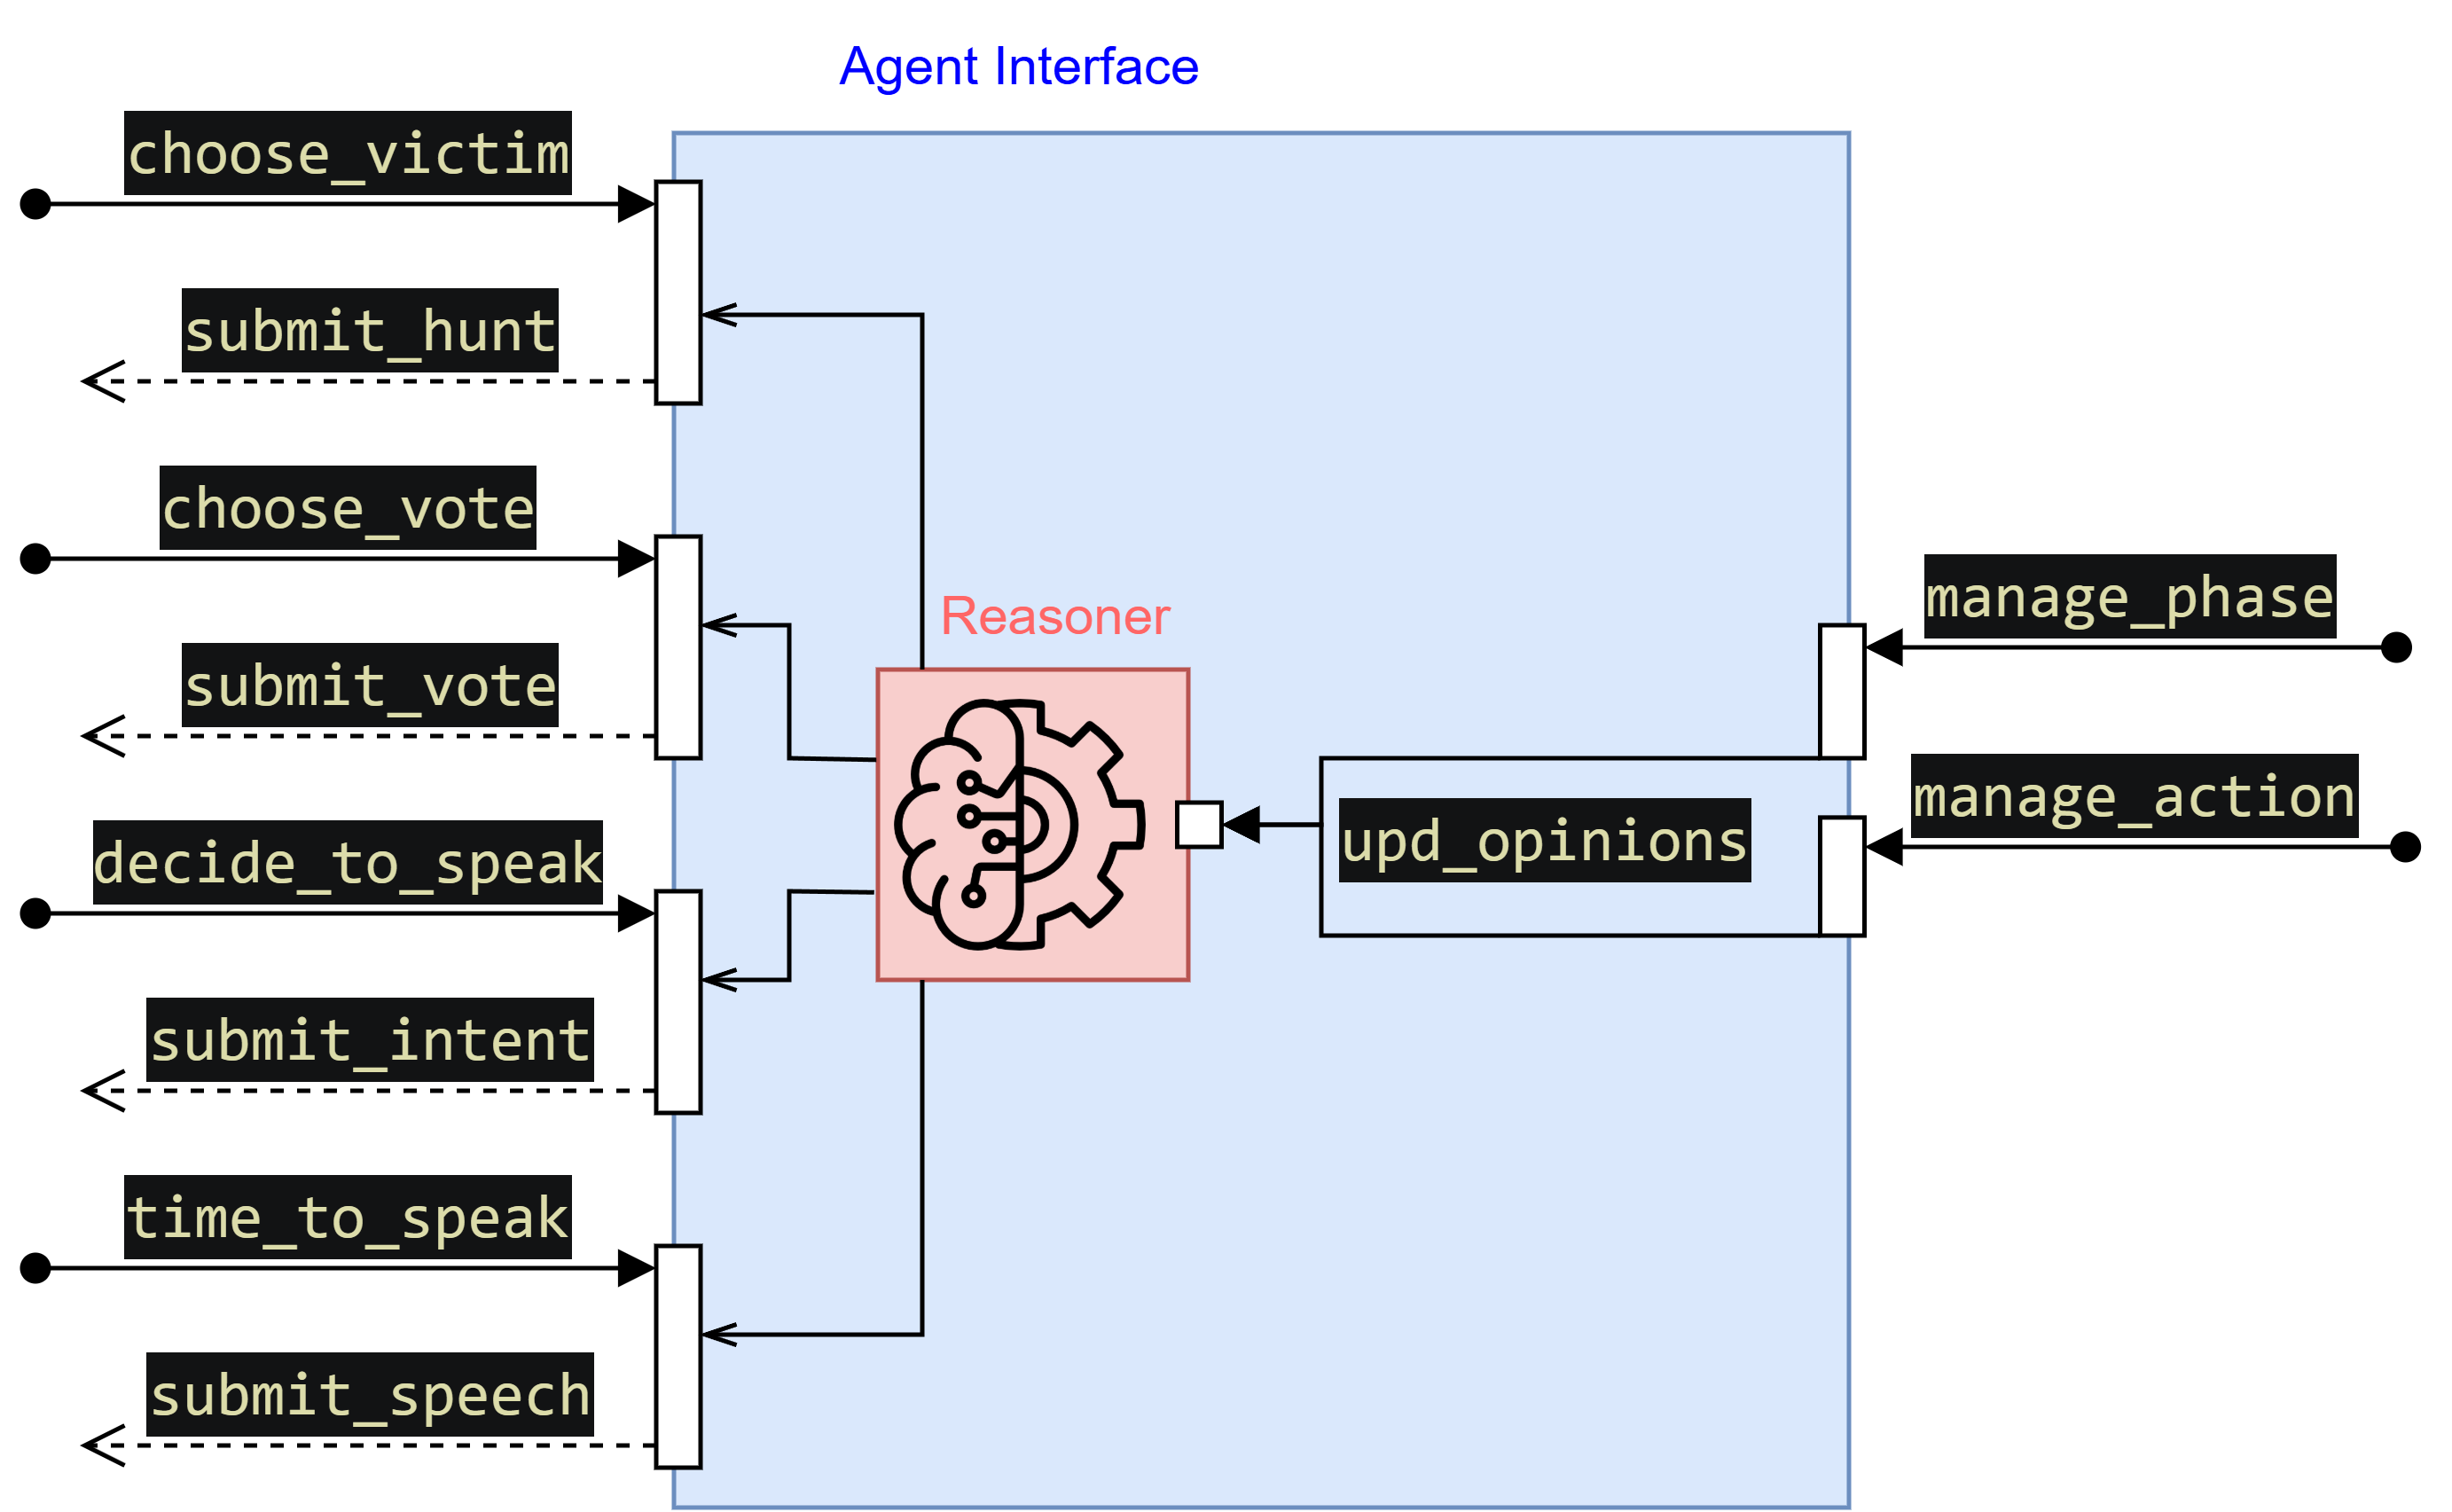
\includegraphics[width=0.8\textwidth]{images/agent_interface.png}
    \caption{Conceptual architecture of the Player Agent, illustrating the decoupling of the fixed network interfaces from the swappable Reasoner logic.}
    \label{fig:agent_interface}
\end{figure}


\paragraph{Decision Execution Interface}
To simplify the interaction protocol, the interface implements a closed-world assumption: every choice must be drawn from an explicitly finite domain. The execution shell must integrate at least 4 plans:
\begin{itemize}
    \item \texttt{choose\_victim}\footnote{The \texttt{choose\_victim} plan is only required if the player holds a \textbf{wolf} role. For standard villagers, the absence of this plan raises no runtime errors, as the Narrator will never explicitly inject this goal for them.} and \texttt{choose\_vote}: Must select  a currently alive player.
    \item \texttt{decide\_to\_speak}: Resolves to a standard intent\footnote{During the resolution phase, the Narrator dynamically casts the a intent into its \texttt{targeted} classification, to properly enforce the discussion phase's speech hierarchy.} (\texttt{yes} or \texttt{no}), or a special \texttt{privileged} flag specifically reserved for human players.
    \item \texttt{time\_to\_speak}: Produces a compound \texttt{speech(Message, Performative(Target))} action. The \texttt{Message} is a textual string, while the \texttt{Performative} must be selected from an enumerated set of valid speech acts (\texttt{accuse}, \texttt{defend}, \texttt{suspect}, \texttt{agree}, \texttt{interrogate}, or \texttt{deflect}) directed at an alive player.
\end{itemize}

When the Narrator inject the agent of its turn, the interface queries the underlying Reasoner to obtain behavior within these rigid boundaries. Once generated, the shell wraps the output into the corresponding submission action to synchronize with the Narrator. 

Furthermore, the architecture could require also a \texttt{guess\_performative} plan, which attempts to extract a valid \texttt{Performative(Target)} tuple from raw textual input if the explicit speech act is missing (further detailed in Section \ref{sec:speech_act_misalignment}).

To prevent temporal misalignment and race conditions across the distributed system, all decisions are strictly dispatched back to the Narrator using the \texttt{sync\_reply(...)} functor (already detailed in Subsection~\ref{subsec:sync-barrier}), as demonstrated in Listing \ref{lst:sync_reply_example}: this implementative choice completely disregard direct communication P2P.

\vspace{1em}
\begin{lstlisting}[frame=single, language=Prolog, caption={An example of a submission helper enforcing synchronization by exclusively replying to the Narrator.}, label={lst:sync_reply_example}]
+!submit_vote(Target) 
  <-.my_name(Me);
    .send(narrator, achieve, sync_reply(vote(Me, Target))).
\end{lstlisting}



\paragraph{State Management Interface} It guarantees the agent's reactivity to the environment. It relies on two passive listener plans: \texttt{manage\_phase} and \texttt{manage\_action}: the goals are injected by the narrator, and the plans does not need to communicate back to the narrator any information (in fact, most of the time the delivered action/phases are ignored altogether). 

Their purpose is to process (mainly by triggering updates to the UI) the incoming events broad casted from the narrator,  and subsequently invoke the \texttt{upd\_opinions(Sender, Action)} hook defined in the Reasoner. As shown in Figure \ref{fig:agent_interface}, this specific hook acts as the bridge to the Reasoner, defining explicit events to update its Belief Base and ensuring the cognitive engine is continuously supplied with an accurate, up-to-date representation of the game's state.


It should be noted that the provided agent interface diagram represents a conceptual simplification. The actual implementation within the Jason environment also integrates extensive conditional hooks to a Graphical User Interface (GUI). When an active UI is present, both the state changes and the decisions trigger corresponding visual updates to dynamically reflect the agent's internal state and actions to the human observer (Section \ref{sec:ui}).


\subsection{Setup and Initialization}
\label{subsec:player-setup}

The orchestration of the simulation begins strictly within the configuration file, \texttt{werewolf.jcm}. To maximize modularity and code reuse, every player in the game is instantiated from a single, universal entry point: the \texttt{players/init\_player.asl} file.

\begin{verbatim}
    agent bob : init_player.asl {
        instances : 1
        beliefs: iam(wolf), reasoner(human)
    }
\end{verbatim}

Within the configuration file, each agent is assigned two mandatory initial beliefs to define their core parameters:
\begin{itemize}
    \item \textbf{\texttt{iam(Role)}:} Dictates their team affiliation, defining them as either a \texttt{wolf} or a \texttt{villager}.
    
    \item \textbf{\texttt{reasoner(Type)}:} Define the cognitive engine, natively accepting values such as \texttt{human}, \texttt{llm}, or \texttt{symbolic}.
\end{itemize}

Upon initialization, the agent executes the \texttt{+!configure\_player} plan, which evaluates these assigned beliefs and orchestrates a multi-step boot sequence. First, the agent resolves the requested cognitive engine via \texttt{+!resolve\_reasoner}; this step introduces robust fallback logic, such as automatically degrading an \texttt{llm} reasoner to a \texttt{symbolic} one if the LLM is disabled. Next, the system configures the appropriate UI bindings (active/spectator, or none at all).

The agent's structural assembly is then handled by a native Jason routing plan, \texttt{+!load\_modules(Role, ActiveReasoner)}; by using the  Jason's \texttt{.include} directives it dynamically inject the precise \texttt{.asl} modules required by the player.

Once the specialized logic and the universal wrappers (statically included at the head of the file) are fully assembled, the agent executes \texttt{+!cleanup\_boot\_memory} to remove all obsolete plans and beliefs (such as those just activated during initialization, or hooks not used by the newly constructed agent).

\paragraph{Easy configuration}
This modular inclusion pattern ensures that the system remains highly scalable and configurable: it is possible to freely adjust the total number of agents, redefine their roles, or completely swap their underlying reasoning engines by exclusively tinkering with the \texttt{werewolf.jcm} configuration file, all without needing to alter any internal Jason code.



\subsection{Personality and Moods (Jason-Pro)}

To model complex social dynamics, the simulation integrates a variation of the \texttt{vesna.ProAgent} architecture, an extension of the standard Jason engine whose original implementation and details can be found at \cite{vesna_pro_toolkit}. By defining a player with a specific ``temper'', it is possible to fundamentally alter its decision-making process without rewriting the underlying AgentSpeak logic. 

\paragraph{Architectural changes} 
In the original \texttt{ProAgent} implementation, the affective state was encapsulated entirely within the Java architectural layer, since it was only utilized as a hidden heuristic for intention selection. To support the  hybrid reasoning models in the game, the architecture was modified to establish \textbf{bidirectional synchronization} between the Java engine and the AgentSpeak layer.

First, methods were introduced to continuously expose the agent's real-time temper to the AgentSpeak belief base, enabling synchronized updates to the User Interface (section \ref{sec:ui}).

Second, while the original engine strictly managed mood updates via static plan annotations such as $$\texttt{@plan\_example[temper([paranoia(0.8)]), effects([stress(-0.3)[mood]])]} $$ new internal actions were added to allow the Jason agent to explicitly overwrite these values. This ensures that the LLM reasoning engine can actively mutate the agent's emotional states in real time in response to external actions and dynamic game events.

Furthermore, to maintain a notation consistent with the \emph{traits} implemented (subsection \ref{subsec:first_order_beliefs}), the domain of both the temper's states and personality values was shifted from the original $[0, 1]$ to $[-1, 1]$.

\paragraph{Personality definition} The cognitive profile is injected directly during the initialization phase within the \texttt{werewolf.jcm} configuration file; within this new architecture, player configuration is thus a direct upgrade of the one defined previously:

\begin{verbatim}
    agent alice : init_player.asl {
        instances : 1
        ag-class: vesna.ProAgent
        temper: temper( 
            paranoia(-0.8), 
            individualism(0.9), 
            stress(0)[mood], 
            exposure(0.5)[mood] )
        strategy: most_similar
        beliefs: iam(wolf), reasoner(llm)
    }
\end{verbatim}

The \texttt{ag-class} directive overrides the default Jason architecture, linking the agent to the custom Java-based affective engine. The \texttt{temper} definition establishes the agent's baseline psychological profile. It distinguishes between static personality traits (\texttt{paranoia(-0.8)}, \texttt{individualism(0.9)}) and dynamic emotional states via the \texttt{[mood]} annotation (\texttt{stress(0)}, \texttt{exposure(0.5)}). 
Finally, the \texttt{strategy: most\_similar} parameter instructs the agent's intention selection to execute the plan whose affective requirements most closely align with the agent's current temper.




\subsection{Epistemic Beliefs as Long-Term World Model}
\label{subsec:first_order_beliefs}

While the \texttt{vesna.ProAgent} architecture is utilized to model the players' internal states (\textbf{self-awareness}), a formal method is still required to maintain a dynamic, long-term, and subjective representation of the external ``world`` (in the context of the game, the other players).

To address this requirement, the implemented solution employs an explicit trait system to model an agent’s \textbf{first-order epistemic beliefs} regarding its peers\footnote{While modeling higher-order beliefs is theoretically possible within the game's context and architecture, this approach was abandoned to prevent a combinatorial explosion in the dimensionality of the belief matrix, which is already sparse by design (as discussed in Section \ref{sec:results}).}.


\paragraph{The \emph{Traits} Matrix}
By assigning specific traits to the other players, the agent effectively generates a dynamic ``belief matrix`` within the its knowledge base. 
The matrix can be visualized explicitly: the rows corresponding to the other players, the columns the specific tracked traits.

\begin{table}[h]
\centering
\begin{tabular}{lccc}
\hline
\textbf{Player} & \textbf{Suspicion} & \textbf{Utility} & \textbf{Influence} \\
\hline
Alice & 0.8 & 0.5 & 0.9 \\
Bob & -0.4 & 0.2 & - \\
Charlie & - & -0.7 & 0.2 \\
Arthur & -0.9 & 0.8 & -0.5 \\
Bella & -0.8 & 0.6 & 0.1 \\
Caleb & 0.7 & - & 0.4 \\
David & - & 0.4 & 0.8 \\
Eve & - & 0.9 & 0.7 \\
Frank & - & -0.5 & - \\
Grace & 0.9 & -0.8 & 0.3 \\
Heidi & 0.6 & 0.3 & 0.5 \\
Ivan & 0.4 & 0.1 & -0.2 \\
Judy & -0.6 & 0.7 & - \\
Kevin & - & 0.5 & 0.6 \\
Leo & 0.0 & 0.0 & - \\
\hline
\end{tabular}
\caption{Player Trait Matrix: the lazy initialization ensures that empty cells contain a value when they will be used.}
\end{table}

This internal representation enables the AgentSpeak interpreter to identify the most suitable target players using customizable heuristics. An application of this approach is detailed in Section \ref{subsec:symbolic-reasoner}, which introduces a symbolic reasoner that directly queries this belief matrix to drive the agent's decision-making process.

\paragraph{Implemented Traits}
The trait framework is designed to be highly modular, allowing to append new heuristics freely without any particular constraint. In the current implementation, each agent keep a matrix where each peer is characterized by 3 traits:

\begin{itemize}
    \item \textbf{Suspicion (Villager specific):} A low level indicates the target is believed to be innocent and trustworthy, while a higher value indicates a strong belief that the target is a wolf.
    \item \textbf{Threat (Wolf specific):} A low level means the target is ignoring the pack or poses no danger, whereas a higher value indicates they are actively attacking the wolves.
    \item \textbf{Utility (Universal):} Evaluates strategic usefulness: a low level defines the target as an obstacle, while a bigger value implies they are actively helpful to the agent's goals.
    \item \textbf{Influence (Universal):} Evaluates social capital: a low level means the target is losing credibility and does not show leadership, while a bigger value denotes that they are highly persuasive and leading the game logic.
\end{itemize}


\subsubsection{Lazy Initialization and Consistency}
To optimize memory usage and accurately simulate initial social uncertainty, the belief matrix employs a lazy initialization implementation. If an agent attempts to query a trait for a specific player that has not yet been formed, the system dynamically generates it on the fly. Rather than starting from an absolute zero, a small amount of Gaussian noise is added to mirror the ``prior knowledge'' that players might possess\footnote{From an implementation perspective, adding random noise to each player's world model ensures stochasticity. This prevents the inherent determinism of a symbolic engine from causing agents to form identical beliefs and, consequently, show uniform behavior.}. 

To ensure mathematical consistency across the reasoning cycle and the UI rendering, all trait values are strictly clamped within the $[-1, 1]$ interval and rounded to two decimal places.

\begin{lstlisting}[frame=single, language=Prolog, caption={Implementation of trait management defined in \texttt{players/first\_order\_beliefs/traits.asl}. The code features lazy initialization of undefined traits using Gaussian noise to introduce stochasticity, alongside an atomic update plan that seamlessly queries (initializing if necessary) and modifies the belief by a given delta.}, label={lst:trait_management}]
    //ensure value in range [Min, Max]
    //define DP decimal places
    clamp(Val, Clamped)
        :-  setting(trait_bounds(Min, Max, DP))
        &   Factor  = 10**DP
        &   TempVal = math.max(Min, math.min(Max, Val))
        &   Clamped = math.round(TempVal * Factor) / Factor.
    
    //MAGIC NUMBERS to add gaussian noise
    add_noise(Mean, StdDev, ClampedResult)
        :-  .random(U1) &   .random(U2)
        &   RealU1 = math.max(0.0001, U1)
        &   Z0 = math.sqrt(-2.0 * math.log(RealU1)) 
               * math.cos(6.28318530718 * U2)
        &   RawVal = Mean + (Z0 * StdDev)
        &   clamp(RawVal, ClampedResult).
    
    //lazy initialization, if not exists
    +?trait(Player, Attr, Value) 
        :   not trait(Player, Attr, _)
        &   setting(trait_bounds(Min, Max, _))
        &   setting(trait_init_noise(StdDev))
        &   add_noise((Min + Max) / 2.0, StdDev, Value)
        <-  +trait(Player, Attr, Value).
    
    //else, simple read
    +?trait(Player, Attr, Value) 
        :   trait(Player, Attr, Value).

    //plan to update a trait
    @upd_trait[atomic]
    +!upd_trait(Player, Attr, Delta)
        <-  ?trait(Player, Attr, CurrentVal);
            ?clamp(CurrentVal + Delta, NewVal);
            .abolish(trait(Player, Attr, _));
            +trait(Player, Attr, NewVal).    
\end{lstlisting}

Furthermore, this dynamic architecture offers high scalability during runtime: theoretically, entirely new trait categories could be defined and queried for a player at any moment without requiring reconfiguration\footnote{However, dynamically introducing new trait types during runtime was intentionally restricted in the final implementation to enforce a ``closed-world assumption''. This constraint is necessary, again, to prevent a combinatorial explosion in the belief matrix's dimensionality.}.



\subsection{Symbolic Reasoner (Jason-Pro)}
\label{subsec:symbolic-reasoner}

With the foundational architecture established, we can define the first type of cognitive engine required for a fully autonomous Multi-Agent System (MAS) simulation. As illustrated before in Figure \ref{fig:agent_interface}, the reasoner must exhibit two primary capabilities: it must continuously store and update information within its internal ``world model``, and it must retrieve this data to govern the agent's decision-making behavior.

As previously defined, this internal world representation is composed of the agent's affective ``self-awareness'' (its temper and personality) and its first-order epistemic beliefs regarding other players. Together, these internal states effectively define the player as a deterministic state machine.

\begin{figure}[H]
    \centering
    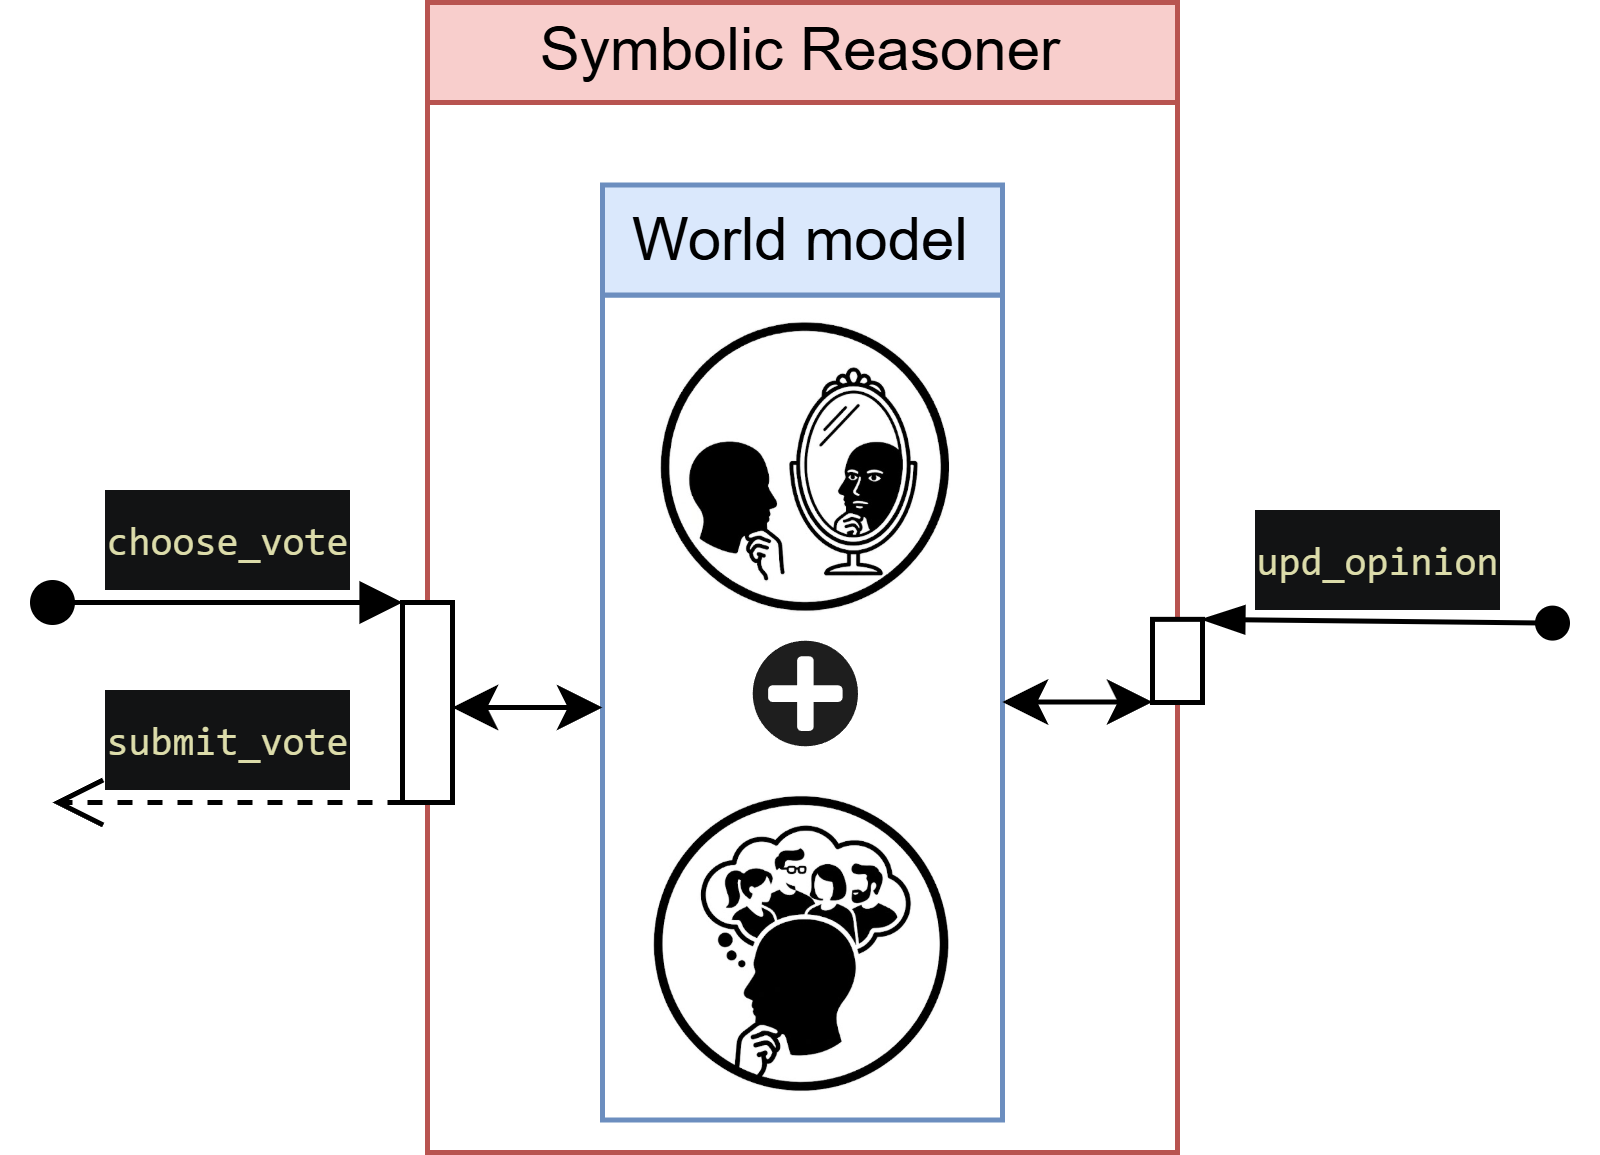
\includegraphics[width=0.6\textwidth]{images/symbolic_reasoner/simplified_symbolic_reasoner.png}
    \caption{Conceptual architecture of the Symbolic Reasoner: at an abstract level, it acts as an interface to query and update the agent's internal world model, which comprises both its \emph{self-awareness} and \emph{first-order epistemic beliefs} about others.}
    \label{fig:symbolic_reasoner}
\end{figure}

The technical implementation of the reasoner's interface, which serves as the execution wrapper for accessing and modifying this internal state, is defined in \texttt{reasoners/symbolic/interface.asl}.

\paragraph{Log retrieval (and Caching)}
For a finer representation of the most recent events, the players can also query the \emph{Narrator} to obtain the last log chunk. Since multi-agent communication in Jason natively brings asynchronous overhead (by forcing the de-scheduling of the active intention), it was also needed to ensure a correct \emph{caching architecture} of the chunks.

When an agent requests a log sequence using the \texttt{+!fetch\_log\_block} plan and the \texttt{cache\_if\_possible} flag, the retrieved data is stored locally in its belief base. A locking mechanism prevents redundant network calls from concurrent requests. To ensure data consistency without continuous polling, the narrator actively invalidates this cache whenever new events modify the historical record.

This logic is integrally implemented in the file \texttt{log\_getter/getter.asl}.

\paragraph{Role-Specific Strategies}
While the player's interface provides a standard execution wrapper, the symbolic reasoner requires role-specific logic. As explained in Subsection \ref{subsec:player-setup},in the player initialization is dynamically loaded the appropriate strategy module (\texttt{strategies/wolf.asl} or \texttt{strategies/villager.asl}). This specialization is crucial, as the two roles exhibit fundamentally different cognitive plans and affective heuristics in response to the exact same game events.


\subsubsection{Updating the Internal State}
As previously discussed, the Reasoner implements its reactivity to events by defining execution plans implementing the \texttt{upd\_opinions(event)} goal. To fully use the capabilites of the \texttt{ProAgent} implementation,is needed to define \textbf{a pool of candidate plans} for each event, as demonstrated in Listing \ref{lst:opinion_pool_example}.

\begin{lstlisting}[frame=single, language=Prolog, caption={Example of the Villager's plan pool used to react to a player's intent to speak. The java engine selects the most suitable reaction based on the agent's temper.}, label={lst:opinion_pool_example}]
@p1[ temper([exposure(0.7)[mood], stress(-0.2)[mood]]), 
     effects([exposure(-0.1)[mood]]) ]
+!upd_opinions(Speaker, intent_to_speak(yes))
    <-  !upd_trait(Speaker, influence, 0.1).

@p2[ temper([paranoia(0.7), stress(0.4)[mood]]),
     effects([stress(0.05)[mood]]) ]
+!upd_opinions(Speaker, intent_to_speak(yes))
    <-  !upd_trait(Speaker, influence, 0.05);
        !upd_trait(Speaker, suspicion, 0.05).

@p3[ temper([paranoia(0.6), stress(0.5)[mood]]), 
     effects([stress(0.1)[mood]]) ]
+!upd_opinions(Speaker, intent_to_speak(no))
    <-  !upd_trait(Speaker, influence, -0.1);
        !upd_trait(Speaker, suspicion, 0.1).

@p4[ temper([individualism(0.7), paranoia(-0.4)])]
+!upd_opinions(Speaker, intent_to_speak(no))
    <-  !upd_trait(Speaker, influence, -0.15).
\end{lstlisting}

By design of the Jason-Pro extension, the reasoning engine evaluates this candidate pool to dynamically select the optimal plan driven by the agent's current \texttt{temper}; at the same time, it processes also the \texttt{effects(...)} annotation, changing the agent's internal mood and updating its overall self-awareness\footnote{To guarantee unbiased plan selection, it is \textbf{required} that all \texttt{temper([...])} annotations within a pool share the exact same dimensionality, since the engine calculates an unnormalized distance metric; the implementation is explained in \cite{vesna_pro_toolkit}, specifically is defined in the file \texttt{src/vesna/ProAgent.java }}.

\begin{figure}[H]
    \centering
    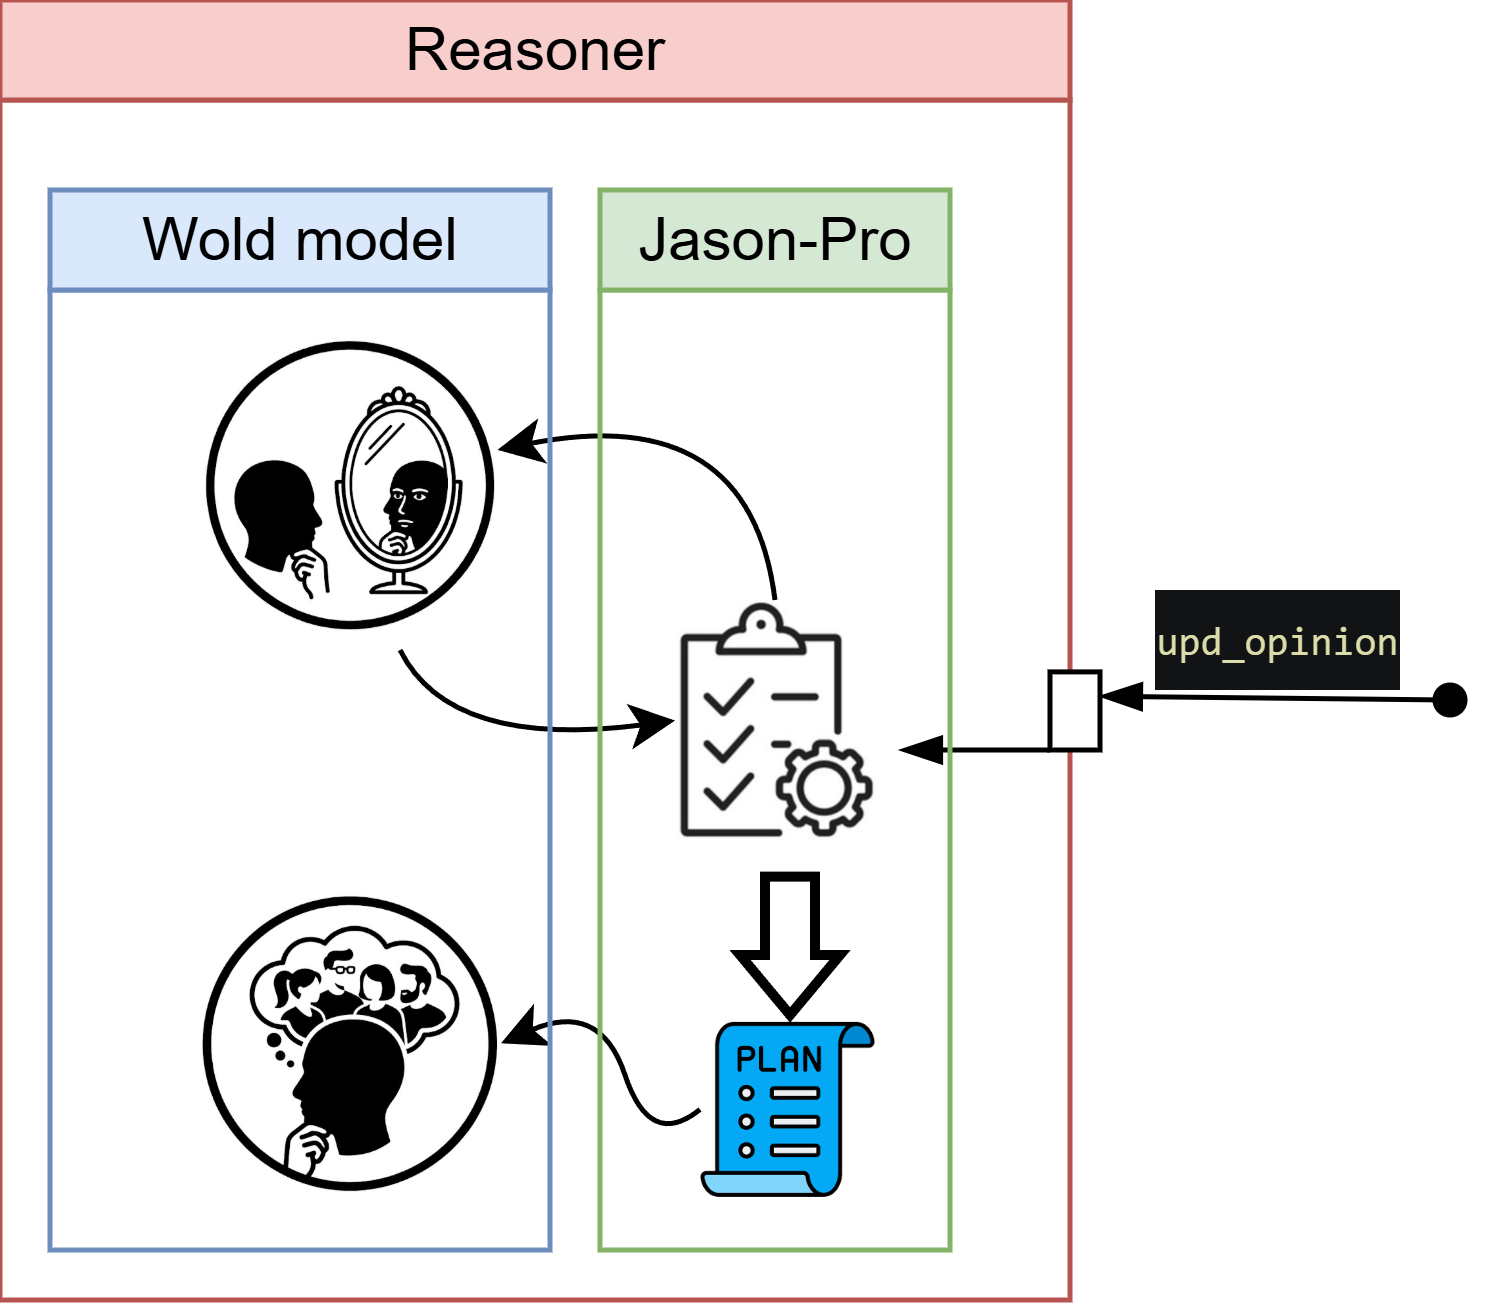
\includegraphics[width=0.6\textwidth]{images/symbolic_reasoner/write_on_symbolic_reasoner.png}
    \caption{Execution pipeline for state updates: external events trigger \texttt{upd\_opinion}, prompting the Jason-Pro engine to evaluate the candidate pool, select a specific plan, and subsequently update both its self-awareness and first-order epistemic beliefs.}
    \label{fig:symbolic_reasoner_write}
\end{figure}

Once selected the plan, executing it applies precise quantitative shifts to the target players' traits, changing the agent's internal belief matrix.


\subsubsection{Querying the Internal State}

\begin{figure}[H]
    \centering
    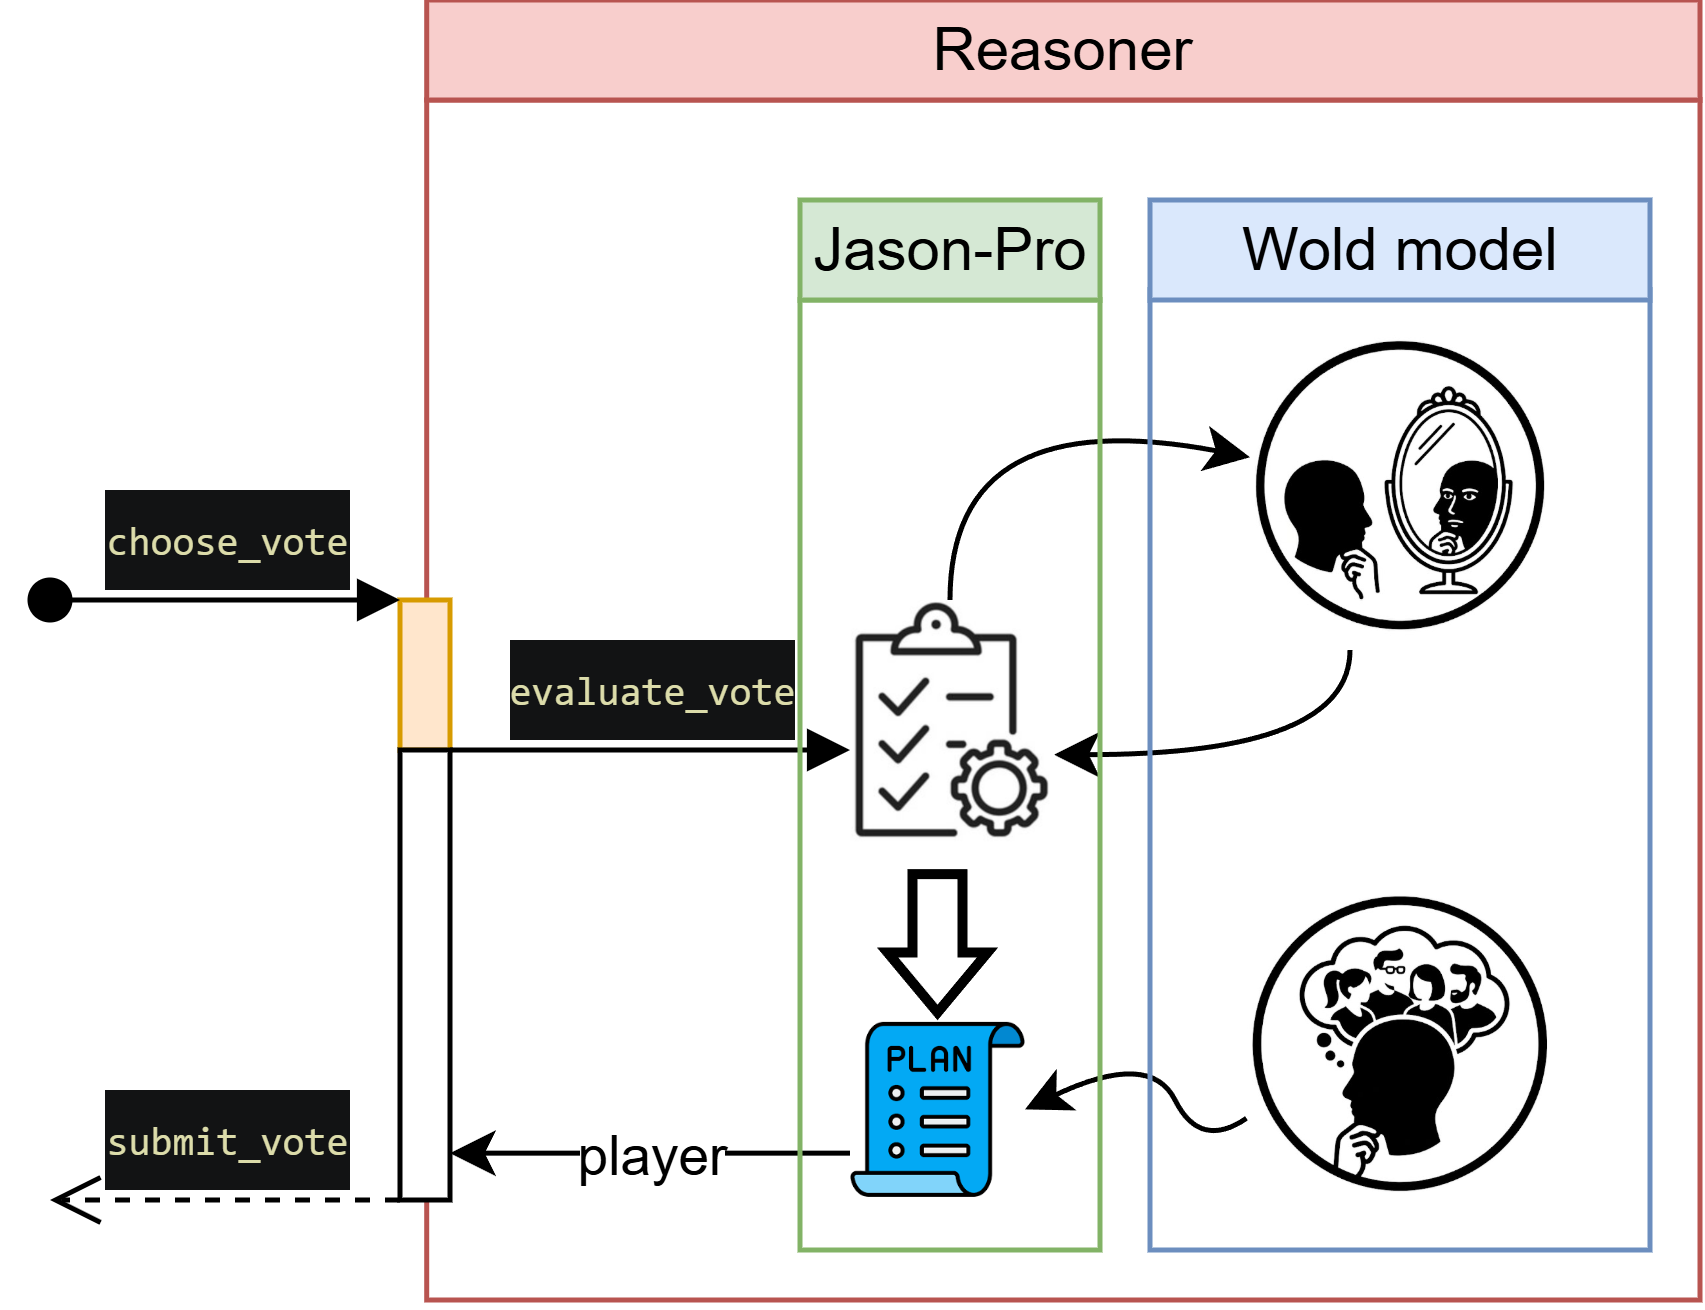
\includegraphics[width=0.6\textwidth]{images/symbolic_reasoner/read_on_symbolic_reasoner.png}
    \caption{Execution pipeline for state querying: the interface delegates decision-making to the reasoner, which selects a plan based on temper and queries the belief matrix to do its choice. Before the selection of the most suitable plan, a random ``artifical delay`` is implemented to ensure that belief base is fully up-to-date.}
    \label{fig:symbolic_reasoner_read}
\end{figure}
The reasoner also can query its belief base to make active decisions (Figure \ref{fig:symbolic_reasoner_read}). 

Because this process uses the same plan's selection pipeline of state updates, decision-making by design can trigger temper shifts, again by using \texttt{effect(...)}.
\begin{verbatim}
    @voting_panicked[ temper([stress(0.8)[mood], paranoia(0.7)]), 
                     effects([stress(-0.5)[mood]]) ]
    +!evaluate_vote(Target) 
        :   other_players(Others) 
        <-  ?select_by_trait(max, suspicion, Others, Target).
\end{verbatim}


To safely extract targets from the raw belief base, the reasoner utilizes the query mechanics defined in \texttt{reasoners/symbolic/utils.asl} (Listing \ref{lst:query_utils}): first is ensured the lazy initialization of the Attr on all the Candidates, then based on that mapping only, a Target is chosen.

\begin{lstlisting}[frame=single, language=Prolog, caption={Implementation of the querying utilities. The wrapper enforces lazy initialization before safely aggregating and extracting the optimal candidate.}, label={lst:query_utils}]
//strategies:  min,max,random
pick_by_strategy(min, [val(_, T) | _], T).
pick_by_strategy(max, Sorted, T) :- Sorted \== [] 
    & .reverse(Sorted, [val(_, T) | _]).
pick_by_strategy(random, Candidates, Target) :- 
    random_target(Candidates, Target).
//fallback for empty list: return self 
pick_by_strategy(_, [], T) :- .my_name(T).

+?select_by_trait(Op, Attr, Candidates, Target)
    <-  //lazy initialization
        for ( .member(P, Candidates) ) 
            { ?trait(P, Attr, _); };        
        .findall(val(V, P), 
            (.member(P, Candidates) & trait(P, Attr, V)),
            List);
        .sort(List, Sorted);
        ?pick_by_strategy(Op, Sorted, Target).
\end{lstlisting}

